%==============================Kapitola: Základy mikroprocesorové techniky====================================
\chapter{Základy mikroprocesorové techniky}
\minitoc
\newpage
  cílem této kapitoly není výklad, zaměřený pouze na jeden typ obvodu, nýbrž zobecnění základních vlastnosti 
  mikropočítačů. Použitá literatura: \cite{Pinker2004}
  
  \section{Základní funkce a části počítače}
    Počítač můžeme funkčně rozdělit na několik základních částí. Je to \textbf{procesor, paměť programu, 
    paměť dat a periferní obvody}. Periferní obvody tvoří velmi rozmanitou skupinu a jejich skladba je 
    závislá na aplikaci počítače. Vždy však jsou přítomny alespoň vstupní a výstupní obvody, které 
    zprostředkují spojení počítače s okolím. Zvláště v případě využití v automatizaci se počítač vybavuje 
    velmi rozsáhlým souborem speciálních jednotek, jako jsou převodníky, čítače a časovače, výkonové výstupy, 
    galvanicky oddělené vstupy a výstupy atd.
    
    \begin{figure}[ht!]   %\ref{MIT:fig_pocitac01}
      \centering
      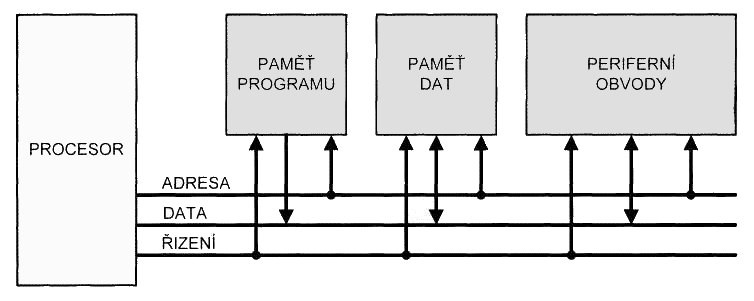
\includegraphics[width=0.7\linewidth]{MCU_arch_basic.png}
      \caption{Zjednodušené schéma počítače}
      \label{MIT:fig_pocitac01}
    \end{figure}

    Vzájemné spojení jednotek je v počítači zásadně zprostředkováno soustavou sběrnic (viz obr. 
    \ref{MIT:fig_pocitac01}). \textbf{Sběrnice} umožňují stavebnicovou koncepci, rozšiřování počítače o další 
    jednotky, a to vše beze změn ve vnitřním zapojení jednotek. Negativní stránkou sběrnice je to, že v 
    každém okamžiku na ni může být připojen jen jeden zdroj dat. Nelze tak např. současně předávat data ze 
    dvou zdrojů ke dvěma příjemcům. Činnost sběrnice je v každém okamžiku řízena jen jednou z jednotek - 
    zpravidla je to procesor, ale v některých případech může dočasně přebírat řízení i jiná jednotka. 
    \begin{itemize}
      \item \emph{Datová sběrnice} slouží k předávání dat a její šířka (tj. počet vodičů) je zpravidla 
      celým násobkem osmi (tj. jednoho byte). Jednotka, připojená na sběrnici, může být zdrojem dat (pak se z 
      ní čte), příjemcem dat (pak se do ní zapisuje), nebo střídavě obojím. Jednotka, která je zdrojem dat, 
      se na datovou sběrnici zásadně připojuje prostřednictvím třístavových členů.
      
      \item \emph{Adresová sběrnice} je nutná pro adresování paměti (případně i jiných adresovatelných 
      obvodů) a pro rozlišování mezi jednotkami, připojenými na datovou sběrnici. Šířka adresové sběrnice 
      určuje maximální počet adres. U osmibitových počítačů má adresová sběrnice šířku nejčastěji 16 bitů, u 
      šestnáctibitových počítačů bývá minimálně 20bitová.
      
      \item Čtení, zápis a další aktivity jednotek jsou řízeny signály \emph{řídicí sběrnice}. Většina 
      řídicích signálů je generována procesorem, ale některé mohou být generovány i ostatními jednotkami, 
      které tak mohou částečně ovlivňovat činnost procesoru - takovéto signály jsou pak na řídicí sběrnici 
      připojeny zpravidla přes členy s otevřeným kolektorem. Řídicích signálů bývá obecně větší počet a 
      podoba řídicí sběrnice je silně závislá na celkové architektuře počítače.
    \end{itemize}
    
    Stručně popišme funkci jednotlivých bloků z obr. \ref{MIT:fig_pocitac01}. Procesor řídí činnost celého 
    počítače. Zajišťuje správné provádění \emph{instrukcí} uložených v paměti programu, zpracovává data v 
    paměti, řídí tok dat ze vstupních obvodů do počítače a jejich zpracování, řídí tok dat z počítače ven 
    přes výstupní obvody. Podle počtu bitů zpracovávaných dat se procesor označuje jako osmibitový, 
    šestnáctibitový, dvaatřicetibitový, atd Je třeba poznamenat, že počet bitů procesoru nemusí být shodný se 
    šířkou datové sběrnice. Tak např. některý 16bitový procesor může využívat jen 8bitovou datovou sběrnici. 
    Vnitřní datové slovo (16 bitů, tj. 2 byte) pak musí samozřejmě být přenášeno na dvakrát. Takovéto řešení 
    je jednodušší z hlediska obvodů i plošného spoje, činnost počítače však bude pomalejší.
    
    \emph{Paměť programu} obsahuje instrukce, jejichž postupným prováděním je realizována požadovaná činnost 
    počítače. Dále často obsahuje různé konstanty a neměnné tabulky, používané v programu. Někdy je program 
    pro danou aplikaci neměnný a pak bývá bezpečně uložen v paměti \emph{ROM} (EPROM, EEPROM, FLASH). Jindy 
    se naopak programy potřebují často měnit. To je případ počítače pro vědecko-technické výpočty. Pak musí 
    být programová paměť typu RAM (Random access memory). Je ovšem nezbytné vyřešit otázku, jak spustit 
    program po zapnutí mikropočítače, kdy paměť RAM má zcela náhodný obsah. Proto se počítač i v těchto 
    případech vybavuje malou programovou pamětí ROM. Po náběhu napájení program začíná zde a vyvolá čtení z 
    velkokapacitní diskové paměti. Její obsah (část operačního systému) se přesune do rozsáhlejší programové 
    paměti RAM. Tento program pak přebírá řízení počítače - komunikaci s operátorem, přesunování dalších 
    programů z diskové paměti, jejich spouštění, atd.
    
    \emph{Paměť dat} zajišťuje dočasné uložení dat, získaných ze vstupních obvodů, uložení mezivýsledků 
    výpočtů apod. Je zásadně typu RAM. Pokud i programová paměť je typu RAM, mohou být případně obě 
    realizovány jedinou společnou paměťovou jednotkou.
    
    \emph{Vstupní a výstupní obvody (l/O - Input/Output)} umožňují počítači komunikovat s vnějším prostředím. 
    Zpravidla obsahují větší počet bran (angl. port), tj. připojovacích míst, rozlišených adresově. Brány 
    mohou být paralelní nebo sériové. Při paralelním přenosu se čte nebo zapisuje najednou celá skupina 
    signálů jako vícebitové slovo (např. 8bitové). Při sériovém přenosu se data přenášejí postupně bit po 
    bitu. Sériový přenos je mnohem pomalejší než paralelní, ale je úspornější co se týče počtu signálových 
    vodičů.
    
    Výše popsaná struktura platí obecně pro všechny počítače. Pokroky v technologii integrovaných obvodů 
    umožnily zmenšení rozměrů a koncentraci mnoha funkcí do jednoho integrovaného obvodu VLSI. Vznikl tak 
    pojem \textbf{mikropočítače} a \textbf{mikroprocesoru}. Je nutné zdůraznit, že předpona „mikro" se 
    vztahuje k fyzický rozměrům obvodů a neznamená omezení funkce. Právě naopak, vysoká integrace umožnila 
    vývoj velmi složitých architektur s vysokým výpočetním výkonem a velkou variabilitou funkcí. Soustředění 
    obvodů na jednom čipu dovoluje zkrátit spoje a tím i zpoždění signálu.
    
    \begin{figure}[ht!] %\ref{MIT:fig_intel4004}
      \centering
      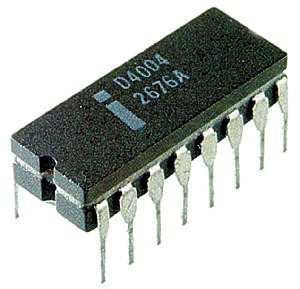
\includegraphics[width=0.5\linewidth]{intel4004.jpg}
      \caption{ První komerčně dostupný 4 bitový procesor 4004 s frekvencí 108kHz od firmy Intel. 
                Obsahoval 2300 tranzistorů a jeho výkon odpovídal 0.06 MIPS (dále obsahoval 16 4bitových 
                registrů, 45 jedno a dvou bitových instrukcí. čtyř úrovňový adresový zásobník a 12bitový 
                programový čítač. Procesor musel být doplněn čtyřmi dalšími podpůrnými obvody 4001 až 4004.}
      \label{MIT:fig_intel4004}
    \end{figure}
    
    Vůbec první procesor s názvem 4004 v podobě jak ho známe dnes představila firma Intel roku 1971. Tento 
    procesor ovšem ke své funkci potřeboval další podpůrné obvody (Intel 4001 až 4OO4). S postupující 
    integrací bylo možné sdružit všechny obvody mikropočítače do jediného integrovaného obvodu. Vznikla tak 
    řada \textbf{jednočipových mikropočítačů}. Zvláště v této skupině počítačů probíhá nejintenzivnější 
    vývoj. Zvětšuje se kapacita paměti programu i paměti dat, rozšiřuje se sestava periferních obvodů. 
    Jednočipový mikropočítač, vhodný pro využití v řízení, je v anglické literatuře označován jako 
    „\textbf{microcontroller}", česky \emph{mikrokontrolér}.
    
    Počítače pronikly do všech oblastí života a jsou součástí měřicích přístrojů, vozidel, audiovizuálních 
    přístrojů, mobilních telefonů, atd. Počítače v těchto aplikacích jsou v anglické literatuře označovány 
    jako „\textbf{embedded computers}", v českém překladu \emph{zabudované} nebo \emph{vložené počítače}.
    
    Vývoj nových typů mikrokontrolérů využívá technologii \textbf{ASIC}, založenou na sdružování a 
    sestavování masek\footnote{slouží v procesu fotolitografie} pro výrobu integrovaných obvodů. Dílčí masky 
    odpovídají osvědčeným, ověřeným jednotkám počítače. Podle potřeby se pak sestaví jádro počítače (procesor 
    a k němu přilehlé obvody), paměti a několik variant sestavy periferních obvodů - vše integrováno na 
    jednom čipu. Vznikají tak \textbf{rodiny mikropočítačů}, které mají společné jádro.
    
    Na rozdíl od rychlého vývoje sestav periferních obvodů a zvyšování kapacity vnitřní paměti je vývoj 
    nových procesorů podstatně konzervativnější. Souvisí to s nutností kompatibility (tj. slučitelnosti) 
    programů po dlouhou dobu. Finanční prostředky, investované do vývoje programů, jsou obrovské a žádný 
    výrobce integrovaných obvodů tuto skutečnost nemůže ignorovat. Modernizace procesoru se děje nejčastěji 
    přidáváním několika málo instrukcí, zvýšením rychlosti, doplněním o specializované obvody. Kompatibilita 
    programů je tak zaručena směrem nahoru (programy pro starší verzi jsou plně použitelné i pro verzi 
    novou), ale ne nutně směrem dolů.
    
    \subsection{Sběrnicové cykly}
      Jak bylo výše řečeno, přenosy dat v počítači probíhají po sběrnicích. Obecný pohled na jednotku, 
      připojenou na sběrnice, dává obr. \ref{MIT:fig_bus_cycle}.
      \begin{figure}[ht!] %\ref{MIT:fig_bus_cycle}
        \centering
        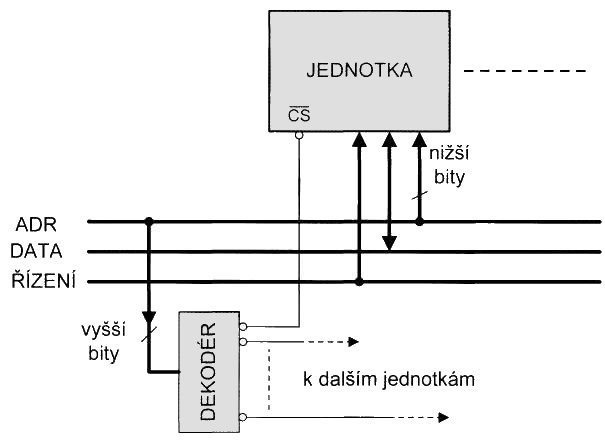
\includegraphics[width=0.7\linewidth]{bus_cycle.jpg}
        \caption{ Připojení jednotky na sběrnice}
        \label{MIT:fig_bus_cycle}
      \end{figure}

      Nejvyšší bity adresy jsou vedeny do \emph{adresového dekodéru}, jehož výstupy (v kódu 1 z N) vybírají 
      jednu z jednotek a povolují její činnost. Pokud je jednotkou samotný integrovaný obvod, bude se zřejmě 
      jednat o jeho vstup CS . Pro jednoduchost budou výběrové signály na výstupech dekodéru takto nazvány i 
      v obecném případě. V jednotce jsou využity zbylé (nižší) bity adresy pro adresování uvnitř obvodů v 
      rámci této jednotky (např. paměti).
      
      Datová sběrnice je obecně dvousměrná a jednotka, připojená na sběrnici, může být jen zdrojem dat (pak 
      se z ní jen čte, např. paměť ROM), příjemcem dat (pak se do ní jen zapisuje, např. výstupní obvody), 
      nebo střídavě obojím (např. paměť RAM). Směr čtení/zápis se rozlišuje vždy z pohledu od procesoru.
      Čtení i zápis jsou řízeny a přesně časovány prostřednictvím signálů řídicí sběrnice. Zatím je označíme 
      jako \texttt{RD} a \textoverline{\texttt{WR}} . Aktivním stavem je zpravidla „L" (low, nízká 
      úroveň) 
      proto jsou v negaci. Řídicích signálů však může být větší počet -např. vstupní a výstupní obvody mohou 
      mít své řídicí signály jiné než paměť.
      
      Posloupnost činností, během kterých dojde právě jednou ke čtení nebo zápisu prostřednictvím sběrnic, se 
      nazývá \emph{\textbf{sběrnicový cyklus} (angl. bus cycle)}. Základními sběrnicovými cykly jsou cyklus 
      čtení z paměti a cyklus zápisu do paměti. Vedle toho mohou existovat i další sběrnicové cykly, jako 
      např. čtení ze vstupních obvodů, zápis do výstupních obvodů, aj. Časování signálů může být v těchto 
      cyklech odlišné.
      
      Pokud má být rychlost procesoru i dalších obvodů počítače využita na maximum, musí být časování velmi 
      přesné. To je zajištěno synchronizací procesoru generátorem hodinových impulzů, řízeným krystalem.

    \subsection{Periferní obvody}
      Periferní obvody tvoří velmi rozmanitou skupinu obvodů, zvláště u počítačů využitých pro řízení. I přes 
      jejich rozmanitost však lze nalézt obecně platné vlastnosti. Velmi často je několik periferních obvodů 
      sdruženo (integrováno) dojedná periferní jednotky např. několik paralelních bran, několik sériových 
      bran, několik čítačů a časovačů, vícekanálový převodník A/Č, apod.
      Zjednodušené schéma periferní jednotky ukazuje obr. \ref{MIT:fig_periferie}.
      \begin{figure}[ht!] %\ref{MIT:fig_periferie}
        \centering
        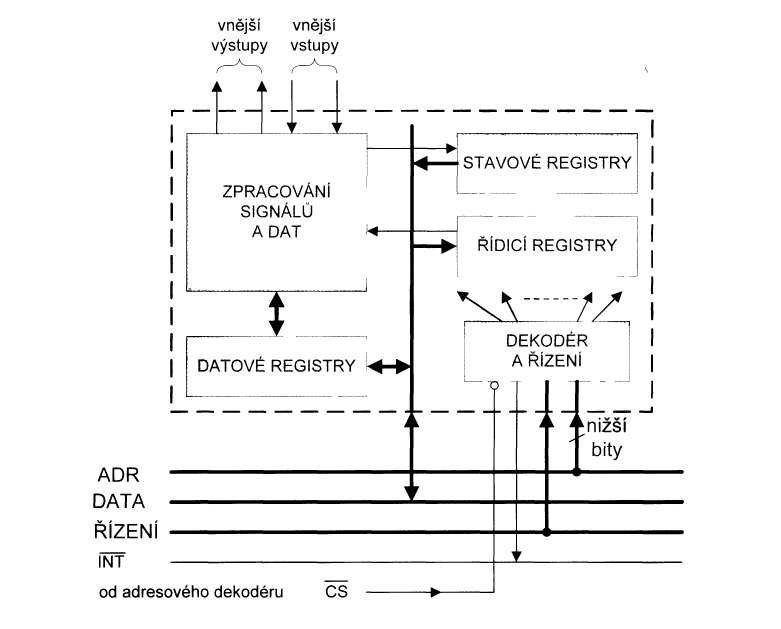
\includegraphics[width=0.7\linewidth]{periferie.jpg}
        \caption{Zjednodušené schéma periferní jednotky}
        \label{MIT:fig_periferie}
      \end{figure}
      
      Jádrem periferní jednotky jsou obvody pro zpracování signálů. To jsou např. čítače, převodníky, nebo 
      třeba jen jednoduché výkonové oddělovací členy. Ze strany datové sběrnice s nimi komunikuje procesor, z 
      druhé strany pak okolí počítače. Jelikož v jednotce bývá sdruženo několik periferních obvodů, jsou data 
      ukládána do několika datových registrů.
      
      Velmi často je nutné činnost těchto obvodů nějak řídit - nastavit cesty signálů, dělicí poměry čítačů, 
      různé vnitřní vazby, apod. K tomu slouží skupina \emph{řídicích registrů}. Dále je třeba zjišťovat stav 
      těchto obvodů - např. přetečení čítače, skončení A/Č převodu, přijetí znaku v sériovém přenosu, apod. K 
      tomu slouží skupina \emph{stavových registrů}. Procesor může prostřednictvím datové sběrnice zapisovat 
      do řídicích registrů a číst stavové registry. \emph{U jednočipových mikropočítačů jsou řídicí a stavové 
      registry seskupeny v jedné oblasti vnitřní paměti}.
      
      Jednotka může vyžadovat obsluhu též prostřednictvím přerušení programu. K tomu slouží jeden nebo více 
      signálů \texttt{INT}. Podnětem k vyvolání přerušení je dokončení požadované operace (dokončení A/Č 
      převodu, přijetí znaku v sériovém přenosu, atd.) nebo případné hlášení chyby (zvláště v komunikačních 
      obvodech). Do jednotky je vedeno několik (nejnižších) adresových bitů pro rozlišení mezi různými 
      datovými, řídicími a stavovými registry. Uvnitř jednotky zřejmě musí existovat ještě lokální adresový 
      dekodér. Signál \texttt{CS} (pokud vůbec existuje) blokuje vždy jen komunikaci s jednotkou ze strany 
      sběrnic, nikdy neblokuje činnost vnitřního jádra, ani vnějších vstupních a výstupních signálů, ani 
      vyvolání přerušení.
      
    \subsection{Adresový prostor}
      Adresový prostor je \emph{množina adres}, na které lze dosáhnout jedním typem sběrnicového cyklu. Tak 
      může existovat \emph{programový prostor, datový prostor, vstupní/ výstupní prostor}, atd. Existuje 
      několik uspořádání adresových prostorů, která úzce souvisejí s architekturou počítače, se složením 
      řídicí sběrnice, a též s instrukčním souborem procesoru.
      
      Adresové prostory lze velmi snadno znázornit, jak ukazuje obr. \ref{fig_MIT:adrspace1}. Jedná se v 
      tomto případě o \textbf{počítač s jediným adresovým prostorem}, do kterého jsou vloženy dílčí prostory 
      - programový, datový a periferní. Adresy rostou směrem zdola nahoru (v některých publikacích je zvolen 
      opačný směr). Co se týče obvodového řešení, je zahrnutí všech obvodů do jednoho prostoru docíleno 
      jedním adresovým dekodérem, který aktivuje vždy jednu skupinu obvodů (např. paměť ROM, paměť RAM, 
      periferní obvody) a společným rozvodem řídicích signálů \texttt{RD} a \textoverline{\texttt{WR}} do 
      všech obvodů (s výjimkou do ROM, kde zřejmě signál \textoverline{\texttt{WR}} pro řízení zápisu 
      nemá smysl). Existují tedy zásadně jen dva sběrnicové cykly - čtení a zápis. Obvodové uspořádání 
      ukazuje obr. \ref{fig_MIT:adrspace1}. K výběru obvodů jsou využity nejvyšší bity adresy. Tato 
      architektura se nazývá \textbf{von Neumannova}. Výhodou je jednoduché řízení obvodů počítače.
      
      \begin{figure}[ht!]
        \centering  
        \begin{tabular}{cc}
          \subfloat[obsazení adr. prostoru]{\label{fig_MIT:adrspace1}
            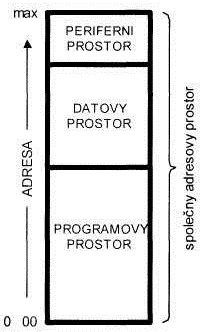
\includegraphics[width=0.14\textwidth]{adresovy_prostor1.jpg}}              &
          \subfloat[obvodové uspořádání]{\label{fig_MIT:adrspace2}
            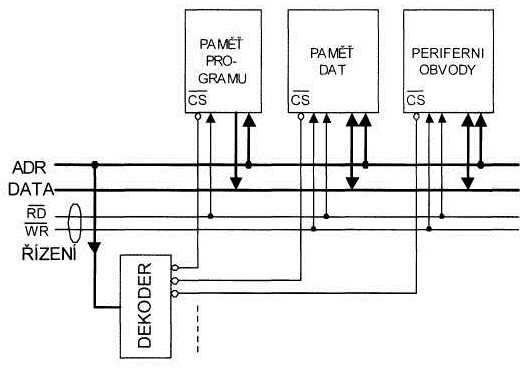
\includegraphics[width=0.32\textwidth]{adresovy_prostor2.jpg}}              \\
        \end{tabular}
        \caption{Počítač s jedním adresovým prostorem}
      \end{figure}
\printbibliography[heading=subbibliography]